\documentclass[a4paper, 12pt]{article}
%\usepackage[utf8]{inputenc} 
\usepackage[frenchb]{babel}
\usepackage{fullpage}
\usepackage[T1]{fontenc} 
\usepackage{graphicx}  
\usepackage[final]{pdfpages}
\usepackage{amsmath, amssymb,amsthm}
\usepackage{algorithm,algorithmic}
\usepackage{listingsutf8}
\usepackage{lmodern}
\usepackage{tikz}
\usepackage{pgfplots}
\usepackage{fancybox}
%\usepackage{slashbox}
\usepackage{makecell}
\usepackage{array, multirow, tabularx}
\usepackage{xcolor}
\setlength{\parskip}{\bigskipamount}

\newtheorem{mydef}{Définition}
\newtheorem{thm}{Théorème}
\newtheorem{lem}{Lemme}
\newtheorem{cor}{Corollaire}
\newtheorem{prop}{Propriété}

\title{Rapport de Méthodes approchées.}
\author{Dyce William, Loukil Amal, Ouazzani-chahdi Sabrina : \\ M1 MOCA}
\date{semestre 2 : 2011-2012}

\begin{document} 

\maketitle

\begin{abstract}
  Le présent document consiste en un mémoire au sujet
  d'exercices à la fois théoriques et pratiques sur diverses
  problèmatiques liées à l'étude de méthodes approchées pour la
  résolution de problèmes NP-difficiles. 
\end{abstract}
\vspace{2cm}
\textit{Travelling salesman's problem :}
\begin{figure}[h!]
\centering
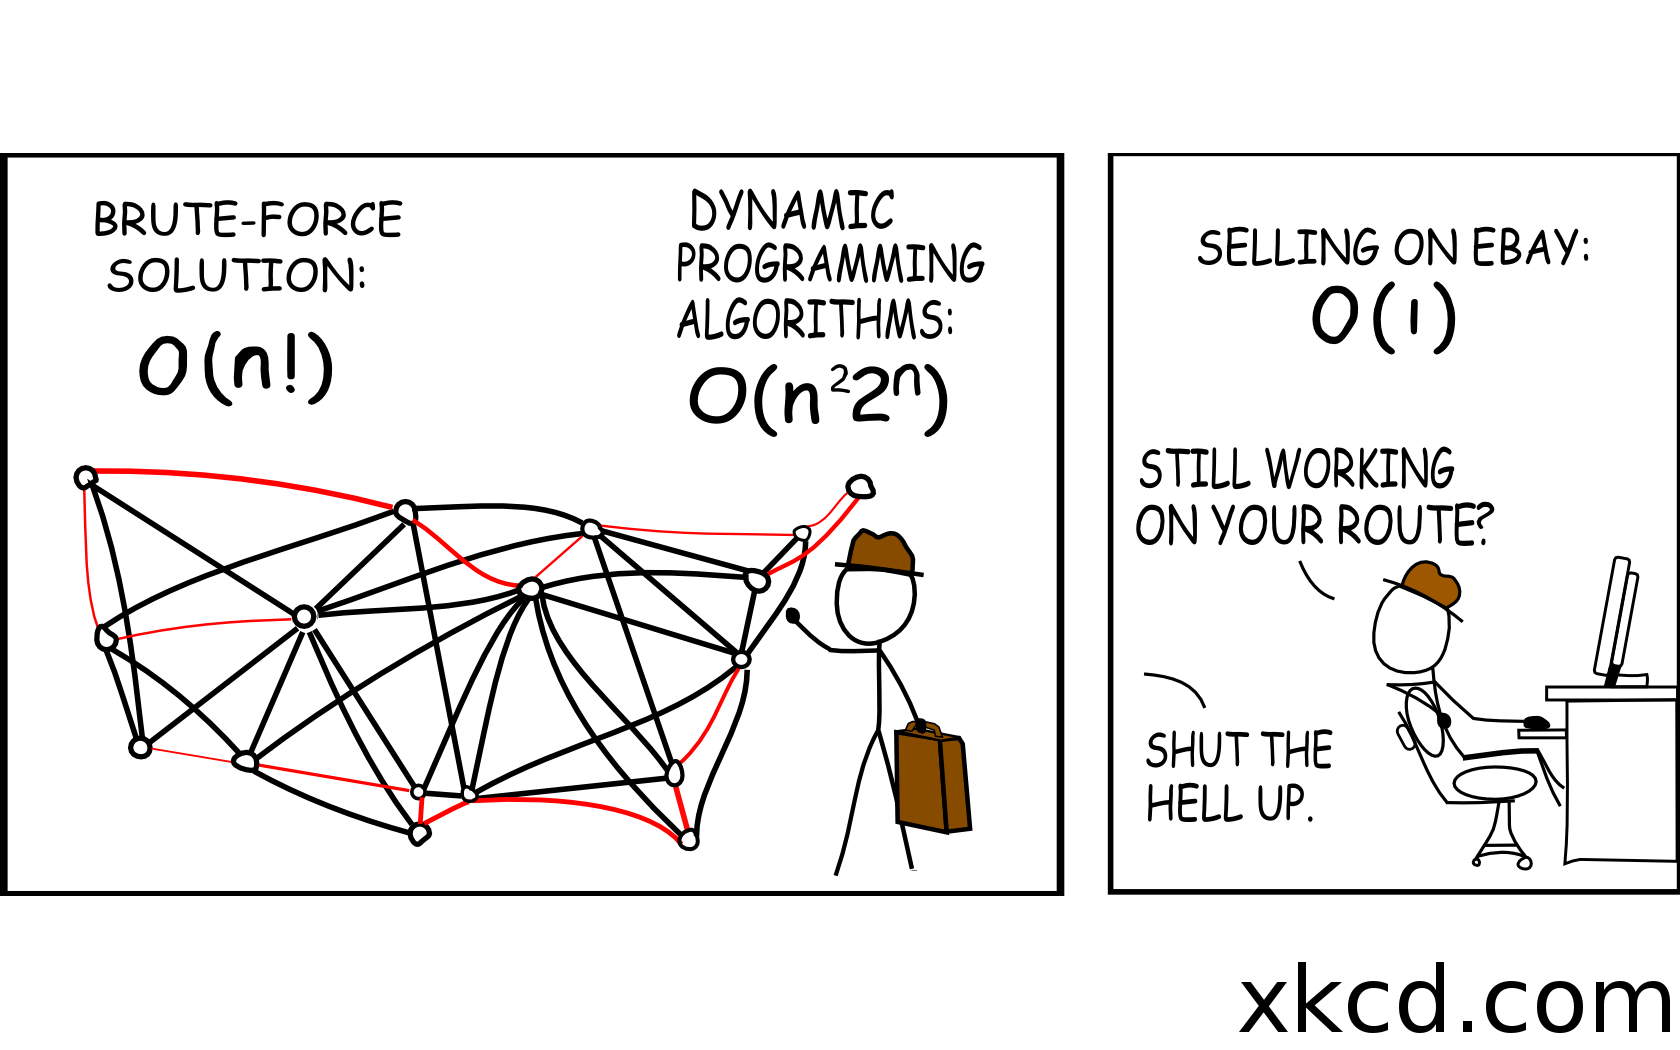
\includegraphics[height = 9cm]{commerce.png}
\end{figure}


\pagebreak

\tableofcontents

\pagebreak

\listoffigures

\listoftables
\pagebreak

\section{Généralités et notations}

\pagebreak

\section{Partie théorique}

\subsection{Programmation linéaire en nombres entiers}

\subsubsection*{Exercice 1}
\paragraph{Question 1}

\begin{itemize}
\item[] a) Le programme linéaire en nombre entier présenté dans
  l'énoncé se justifie de la manière suivante~:
\begin{itemize}
\item $x_j \in \{0,1\}, j=1..n$ car on a le choix binaire entre prendre un
  sommet (donc le compter avec 1), ou ne pas le prendre (ne pas le
  compter avec 0, élément neutre de l'addition). Il y a bien
  évidemment n sommets, d'où l'indexation de 1 à n.
\item $min z = \sum^n _{i=1} x_i$ car on souhaite minimiser le nombre
  de sommets pris.
\item $x_r + x_s \geq 1$ car au moins un sommet doit être pris pour
  couvrir une arête.
\end{itemize}
Ces trois conditions décrivent donc bien le problème de la couverture minimale.
\item[] b) Le cas du triangle est un contre-exemple qui contredit cette
égalité. En effet (cf le dessin ci-dessous) le fait de
choisir l'arête $AC$, par exemple, empêcherait de sélectionner les
autres arêtes (sous peine de violer la contrainte d'égalité) alors
qu'un sommet resterait insaturé. Cette condition doit donc être
élargie à une inégalité.
\begin{figure}[!ht]
\begin{center}
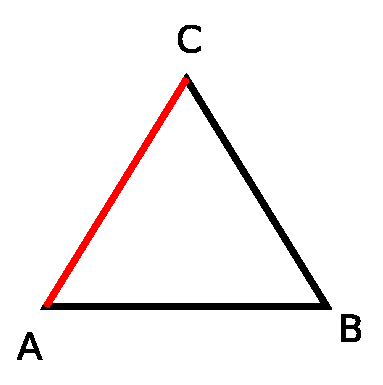
\includegraphics[height=3cm]{../images/triangle.eps}
\end{center}
\caption{Pourquoi on ne peut pas avoir $x_r + x_S = 1$.}
\end{figure}
\item[] c) Montrons par l'absurde que le programme linéaire en nombres
  entiers est une borne inférieure de toute solution optimale.
\begin{proof}
Supposons que pour une instance donnée, on ait une solution optimale
de vertex cover qui soit meilleure que PLNE. Cela veut donc dire que
PLNE garde au au moins un sommet <<~en trop~>>. Or PLNE devrait
minimiser le nombre de sommets et le simplexe est adéquat. Le résultat
est donc absurde et contredit notre hypothèse de départ.
\end{proof}
\item[] d) Nous allons ici montrer de deux manières différentes que la
  relaxation des contraintes d'intégrité implique $x_r \geq
  \frac{1}{2}$ ou $x_s \geq \frac{1}{2}$.
\begin{itemize}
\item Première démonstration.
\begin{proof}
On veut, malgré la relaxation des contraintes d'intégrité, conserver
l'inégalité $x_r + x_s \geq 1$. Ainsi, on a $\neg (x_r + x_s < 1)$
d'où $\neg (x_r < \frac{1}{2} \wedge x_s < \frac{1}{2})$, et donc
($x_r \geq \frac{1}{2} \vee x_s \geq \frac{1}{2}) $ de par la loi de
De Morgan.
\end{proof}
\item Deuxième démonstration.
\begin{proof}
On sait que $A \Rightarrow B \equiv \neg A \vee B$. 
Or, pour respecter l'inégalité $x_r + x_s \geq 1$, on a $(x_r <
\frac{1}{2} \Rightarrow x_s \geq \frac{1}{2})$. On a ainsi $(x_r \geq
\frac{1}{2} \vee x_s \geq \frac{1}{2})$. 
\end{proof}
\end{itemize}
\item[] e) Montrons que l'algorithme 1 conduit à un algorithme
  approché avec une performance relative de de deux. 
\begin{proof}
Soit $C^{*}$ une solution optimale du problème de la couverture de
sommet. Soit $C$ la solution donnée par l'algorithme. 
$x_r=x_s=\frac{1}{2}$. Après la phase d'arrondi $x_r=x_s= 1$. D'où $
OPT = \frac{approche}{2}$.
En effet, on a pour exemple de pire des cas un carré, cf figure
ci-dessous.
\end{proof}

\begin{figure}
\begin{center}
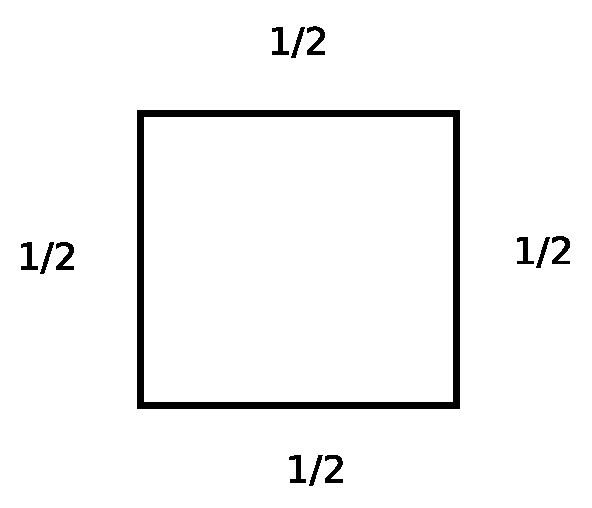
\includegraphics[height=3cm]{../images/carre.eps}
\end{center}
\caption{Pire des cas pour l'algorithme 1}
\end{figure}

\item[] f)
\begin{itemize}
\item i)
Le programme linéaire correspondant à rajouter un poids aux arêtes au
problème du vertex cover est le suivant~:
\begin{equation}
\begin{cases}
min \sum_{i=1}^n w_{i, j}x_i \\
x_r + x_s \geq 1 \\
x_i \in \{ 0, 1 \} \\
\end{cases}
\end{equation}
\item ii)
\begin{equation}
\begin{cases}
min w^Tx \\
A^Tx \geq 1 \\
x_j \in \{0, 1\} \\
\end{cases}
\end{equation}
avec A matrice d'incidence sommets-arêtes.
\item iii) \begin{proof}
$x_i^*\geq \frac{1}{2} \Rightarrow x_i = 1$ \\
$x_i \leq 2x_i^*$ \\
$\Rightarrow C_{PLNE}=\sum x_iw_i \leq (2x_i^*)w_i \leq 2C_{opt}$ \\
\end{proof}
\end{itemize}
\end{itemize}

\paragraph{Question 2}

\begin{itemize}
\item[] a) Montrons que l'algorithme 2 est 2-approché.
\begin{proof}
Soit $C^{*}$ une solution optimale du problème de la couverture de
sommet. Soit $C$ la solution donnée par l'algorithme. 
\begin{itemize}
\item[] $|M| \leq C^{*}$ car deux arêtes adjacentes peuvent être
  couvertes par un même sommet.
\item[] $C^{*} \leq C = 2 |M|$ car une arête a deux sommets.
\item[] On a donc $\frac{C}{C^{*}} \leq \frac{2|M|}{|M|} = 2$.
\end{itemize}
\end{proof}
\item[] b) Il suffit de prendre $C_4$.
\item[] c) 
\begin{itemize}
\item[] Dans le pire des cas donné à la figure 1, l'algorithme renvoie
  une solution $C$ de taille 8. Or la solution optimale $C^*$ pour cette
  instance est de taille 5. En effet, aucun des sommets de plus haut
  degré n'est inclus dans $C^{*}$. Le choix du sommet de plus haut
  degré n'est donc pas une bonne heuristique. 
\item[] En revanche, on peut remarquer que cet algorithme trouve la
  solution optimale sur $C_4$ (qui était le cas limite de l'algorithme 2).
\end{itemize}
\end{itemize}


\subsubsection*{Exercice 2}
\paragraph{Question 1}

Nous proposons la modélisation suivante en programmation linéaire en
nombres entiers pour le problème de la couverture d'ensembles~:
\begin{equation}
\begin{cases}
min \sum_{j=1}^m w_j s_j\\
\sum_{j=1}^{m} s_{j} \geq 1 \\
s_i \in \{0,1\} \\
\end{cases}
\end{equation}
avec $s_j = 1$ si l'ensemble $S_j$ est choisi, 0 sinon.

Proposition sous forme  d'écriture matricielle, avec M matrice
d'appartenance d'un élément $e_i$ à un ensemble $S_j$~:

\begin{equation}
\begin{cases}
min \sum_{j=1}^m w_j x_j\\
\forall i \in \{1, \dots n \} \sum_{j=1}^{m} M_{ij}x_{j} \geq 1 \\
\forall i \in \{1, \dots n\} x_i \in \{0,1\} \\
\end{cases}
\end{equation}
avec $x_j = 1$ si l'ensemble $S_j$ est choisi, 0 sinon.

\paragraph{Question 2}
 Dans un programme en nombre réels, on a plutôt$ s_j \in [0,1]$. Nous
 proposons donc la procédure d'arrondis suivante sur les $s_j$~:
\begin{itemize}
\item Si $s_j \geq \frac{1}{f}$ alors $s_j = 1$,
\item si $s_j < \frac{1}{f}$ alors $s_j = 0$.
\end{itemize}

\paragraph{Question 3}

La procédure d'arrondie précédente garantie une solution réalisable
car elle respecte toutes les contraintes de la modélisation énoncée à
la question 1.

\begin{proof}
Soit $e$ un élément quelconque de $E$. $e$ appartient à au plus $f$ ensembles donc $\sum\limits_{e \in S_{i}} x_{s} \geqslant 1$. Donc $x_{s} \geqslant \frac{1}{f}$ et donc $e$ est couvert.  
\end{proof}

\paragraph{Question 4}

Montrons que le problème de la couverture d'ensemble possède un
algorithme $f$-approché.

\begin{proof}
Soit $C^*$ une solution optimale pour le problème de la couverture
d'ensemble, soit C la solution renvoyée par un algorithme
$f$-approché.

$C^* \geq  \sum_{i=1}^n w_{e_i}$ car deux éléments peuvent appartenir à un même sous-ensemble.
$C \leq f * \sum_{i=1}^n w_{e_i}$ car un élément appartient a au plus $f$ sous-ensembles \\

On a donc $\frac{C}{C^*} \leq f$.
\end{proof}

\paragraph{Question 5}

Quand $f_i = 2$, $e_i$ appartient à deux sous-ensembles. On retrouve
donc le problème de la couverture d'arêtes (les éléments) par des
sommets (les sous-ensembles) (vertex cover).


\subsubsection*{Exercice 3}
\paragraph{Question 1}Le programme linéaire en nombres entiers qui modélise le
  problème du couplage maximum de poids minimum est le suivant.
  (notons $u_{ij}$ les arêtes du graphe)
Notons que $u_{ij} \in \{0, 1\}$ car on prend une arête ou on ne la
prend pas.

\begin{equation}
\begin{cases}
min \sum w_{ij} u_{ij} \\
\forall x_{ij} \in E ~ \sum u_{i' j'} = 1 \\
 x_{i' j'} \in adj(x_{ij}) \cup \{ x_{ij} \} \\
\end{cases}
\end{equation}

En effet, soit $\{ i, j \}$ une arête qui appartient à un couplage
$M$. Par définition, $\Gamma^{-1}(i) $ et $\Gamma^{+1}(j)$
n'appartiennent pas à $M$.

\paragraph{Question 2}

Pour obtenir un couplage de poids minimum, on doit plutôt choisir des
arêtes de valuation $\epsilon$.

\paragraph{Question 3}
\paragraph{Question 4}
\paragraph{Question 5}
La formulation initialement proposée n'est pas pertinente car elle ne
couvre pas tous les cas. On peut ainsi considérer les contre-exemples
suivants~: TODO !

\subsection{Problèmes appartenant à la classe APX}

\subsubsection*{Exercice 4}
\paragraph{Question 1}
La complexité est de $O(m(n+m))=O(n^4)$ car~:
\begin{itemize}
\item La taille de la coupe augmente d'un sommet à chaque tour, donc
il nous faut $m$ étapes pour trouver la coupe maximum.
\item À chaque tour, on rajoute un également toutes les arêtes
incidentes au sommet rajouté.
\end{itemize}

\paragraph{Question 2}
Montrons que le taux d'approximation est de 2~:
\begin{proof}Soit $(Y_1,Y_2)$ la coupe approximatif. Supposons pour $\Gamma(x)$ l'ensemble des sommets voisins d'un sommet x~:

$\exists x \in Y_1 \text{ | } \Gamma(x) \cap Y_1 > \Gamma(x) \cap Y_2$

Dans un tel cas le déplacement du sommet x dans $Y_2$ augmenterai la valeur de la coupe, donc l'algorithme approché ne l'aurait jamais gardé dans $Y_1$. Notre supposition est donc absurde. Nous avions au contraire~:

$\forall x \in Y_1 \text{ | } \Gamma(x) \cap Y_1 \leq \Gamma(x) \cap Y_2$

Le même raisonnement tient pour les sommets de $Y_2$, donc globalement au pire la moité des arrêtes doivent traverser la coupe, soit \mbox{$(Y_1,Y_2) \geq \frac{|E|}{2}$}. Or même la coupe optimale est borné par $|E|$, donc $\frac{(Y_1,Y_2)}{(Y_1,Y_2)^*} \geq 2$, \emph{quod erat demonstrandum}.
\end{proof}

\paragraph{Question 3}

Nous pouvons construire l'instance ci-dessous pour laquelle la borne de
deux est atteinte. 
***************************************
***************************************
**************************************
TODO -- FINIR: énoncer la coupe optimale versus la coupe donné par l'algorithme, montrer que l'un est deux fois l'autre.

\begin{figure}[h!]
\centering
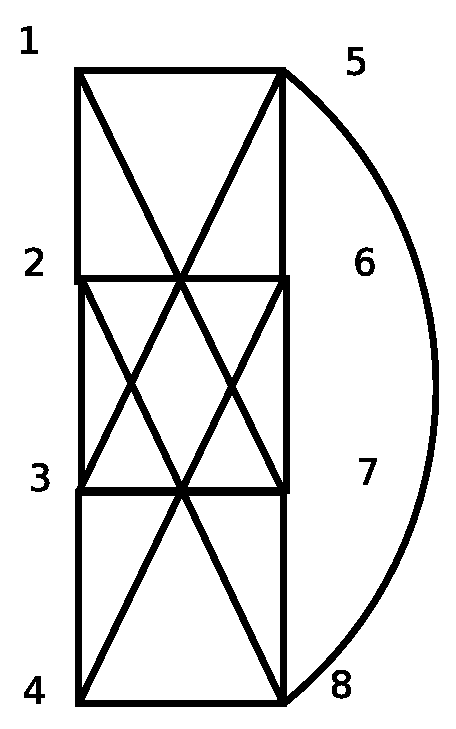
\includegraphics[height = 4cm]{../images/exo4.eps}
\caption{Instance où la borne de $2$ est atteinte, exercice 4}
\end{figure}


\subsection{Constructions de PTAS}

\subsubsection*{Exercice 5}
\paragraph{Question 1}

\paragraph{Question 2}
On suppose que $r < 2$
\begin{itemize}
\item a) Montrons que $w(Y_{1}) - L \leqslant \frac{p(a_{h})}{2}$\\
On a $w(Y_{1})$ - $p(a_{h})$ $\leqslant$ $w(Y_{2})$. On ajoute $w(Y_{1})$ de chaque côté, on obtient 2$w(Y_{1})$ - $p(a_{h})$ $\leqslant$ $w(Y_{2})$ + $w(Y_{1})$ et par suite 2$w(Y_{1})$ - $p(a_{h})$ $\leqslant$ 2L ce qui nous donne $w(Y_{1})$ - L $\leqslant$ $\frac{p(a_{h})}{2}$.
\item b) En insérant l'objet $a_{h}$ dans $w(Y_{1})$ durant la première phase de l'algorithme, on obtient une solution optimale. 
\item c) Si l'objet $a_{h}$ est inséré dans $w(Y_{1})$ durant la seconde phase, c'est à dire que le poids de l'objet  $p(a_{h})$ $\leqslant$ $p(a_{j})$ puisque les objets sont triés par ordre décroissant.\\
Montrons ici que 2L $\geqslant$ $p(a_{h})$ (k(r)+1).
Précédons comme suit:\\
On a $p(a_{h})$ $\leqslant$ $p(a_{j})$ et par suite $\sum_{j=1}^{(k(r)+1)} p(a_{h})$ $\leqslant$ $\sum_{j=1}^(k(r)+1)} p(a_{j})$ or $\sum_{j=1}^{(k(r)+1)} p(a_{j})$ $\leqslant$ W(A) et donc (k(r)+1)$p(a_{h})$ $\leqslant$ W(A) = 2L. 
\item d) $m^{*}$ $\geqslant$ L
\item e) Montrons que le ratio est majoré par $r$.\\
On a $w(Y_{1})$ $\geqslant$ L, servons nous du résultat trouvé dans la question $d$ on a $m^{*}$ $\geqslant$ L.\\
$\frac{1}{m^{*}}$ $\leqslant$ $\frac{1}{L}$, multiplions par $w(Y_{1})$ de chaque côté, on obtient $\frac{w(Y_{1})}{m^{*}}$ $\leqslant$ $\frac{w(Y_{1})}{L}$.\\
On a donc $\frac{w(Y_{1})}{m^{*}}$ $\leqslant$ $\frac {L + \frac {p(a_{h})}{2}}{L}$ $\leqslant$ $1 + \frac{p(a_{h})}{2L}$ $\leqslant$ $1 + \frac{1}{(k(r)+1)}$ $\leqslant$ $1 + \frac{1}{\frac{2-r}{r-1}+1}$ $\leqslant$ $r$
\end{itemize}
\paragraph{Question 3}
La complexité de l'algorithme est: 
\begin{itemize}
\item nlogn pour le trie des objets 
\item $2^{k(r)}$ pour la partition des objets.
\end{itemize}
Donc, la complexité est de $2^{k(r)}$ +  nlogn


\subsubsection*{Exercice 6}
\paragraph{Question 1}
\begin{itemize}
\item a) $nlogn+n = O(nlogn)$
\item b) Si $j = 1$ alors $cost(T) + w_{2} \geqslant B$ et donc $cost(T) \geqslant \frac{B}{2}$.\\
Si $j \geqslant 2$ alors $\sum_{i=1}^{j} W_{j} + W_{j+1} \geqslant B$, c'est à dire $\sum_{i=1}^{j} \geqslant W_{j+1}$ et donc $cost(T) > \frac{B}{2}$.
\item c)  $s^{*} \geqslant B$ et $S \geqslant \frac{B}{2}$\\
$\frac{1}{S} \leqslant \frac{2}{B}$ et donc $\frac{S^{*}}{S} \leqslant 2$.
\end{itemize}

\paragraph{Question 2}
\begin{itemize}
\item a) L'algorithme $2$ admet une complexité de $O(n^{k+1})$ car ~:
\begin{itemize}
\item pour étendre $S$ à $S^*$ on a un coût de $O(nlogn)$~;
\item les ensembles $S$ de taille maximale $k$ sont créés avec un coût
de k parmi n, c'est à dire en $O(n^k)$.
\end{itemize}
\item b)
\begin{itemize}
\item i) Si $p \leq k$ alors on est à l'optimal (puisqu'on s'est
arrêtés avant).
\item ii)
\begin{itemize}
\item A) Si $P^*=M$ alors c'est que la solution est optimale.
\item B) Montrons que $\exists i_q > i_k \geq k$ tel que
$cost(P^*)+w_iq > b \geq cost(M)$.
\begin{proof}
Par définition de l'optimalité, on a $cost(M) \leq b$. $k$ est
l'indice associé à la solution optimale, par définition de la
notation. \\
$cost(P^*) \leq b$ mais $cost(P^*) + w_{i_q} > b$ car sinon $w_{i_q}$
aurait déjà fait partie de la solution (on a $i_q > i_k$). 
\end{proof}
\item C) Montrons que $w_{i_q} \leq \frac{cost(M)}{k+1}$.
\begin{proof}
Si ce n'était pas le cas, on pourrait rajouter $w_{i_q}$ dans
notre solution. En effet, la fraction $\frac{cost(M)}{k+1}$ est
l'espace qu'il reste jusqu'à la solution optimale en prenant un objet
de plus que ce qu'on a pris jusqu'à présent.
\end{proof}
\item D) Évaluons le ratio $R(I, \epsilon)
= \frac{cost(M)}{cost(P^*)}$. \\
TODO
\end{itemize}
\end{itemize}
\end{itemize}


\subsection{Utilisation de méthodes exactes}

\subsubsection*{Exercice 7}
\paragraph{Sur le problème de la partition}

\begin{itemize}
\item a) La condition nécessaire sur la somme des poids des $n$ objets
  est la suivante~: on veut $\sum_{a \in A'} p(a)= \sum_{a \in A
    \backslash A'}p(a)$
\item b) 
\begin{itemize}
\item i) La formule qui lie les lignes $i$, $i-1$ et $p(a_i)$ est $A_i
  := A_{i-1} \cup A_{i, p(a_i)} \cup A_{i-1}+p(a_i)$ avec
  $A_{i-1}+p(a_i) \leq P$.
\item ii) Construisons le tableau à partir de l'exemple donné:
\begin{table}[h!]
\centering
	\begin{tabular}{|c|c|c|c|c|c|c|c|c|c|c|c|c|c|c|c|c|c|}
    \hline
     i $\diagdown$ p & 0 & 1 & 2 & 3 & 4 & 5 & 6 & 7 & 8 & 9 & 10 & 11 & 12 & 13 & 14 & 15 & 16 \\
    \hline
   1 & 0 & 0 & 0 & 0 & 0 & 1 & 0 & 0 & 0 & 0 & 0 & 0 & 0 & 0 & 0 & 0 & 0 \\
     \hline
	2& 0 & 0 & 0 & 0 & 0 & 1 & 0 & 0 & 0 & 1 & 0 & 0 & 0 & 0 & 1 & 0 & 0 \\
   \hline
	3 & 0 & 0 & 0 & 1 & 0 & 1 & 0 & 0 & 1 & 1 & 0 & 0 & 1 & 0 & 1 & 0 & 0 \\
	\hline
	4 & 0 & 0 & 0 & 1 & 0 & 1 & 0 & 0 & 1 & 1 & 0 & 1 & 1 & 1 & 1 & 0 & 0 \\
	  \hline
	5 & 0 & 0 & 1 & 1 & 0 & 1 & 0 & 1 & 1 & 1 & 1 & 1 & 1 & 1 & 1 & 0 & 0 \\
	\hline
	6 & 0 & 0 & 1 & 1 & 0 & 1 & 0 & 1 & 1 & 1 & 1 & 1 & 1 & 1 & 1 & 0 & 0 \\
	\hline
\end{tabular}
\caption {Remplissage du tableau sur l'exemple donné}
\end{table} 
\item iii) Nous proposons les deux algorithmes ci-dessous.
\begin{algorithm}[t]
\caption{Algorithme général}
\label{algoexo7}
\begin{algorithmic}[1]
\STATE $P_1 := \emptyset $,  $P_1 := \emptyset $
\FOR{$i=1 \to n$}
\WHILE{$P_1 < P$ et $P_2 < P$}
\STATE remplir $A_i$ en utilisant la formule présentée avant
\STATE faire Test
\IF {$A(i,j) == 1$}
\STATE $A(i,j):=0$
\ENDIF
\ENDWHILE
\ENDFOR
\end{algorithmic}
\end{algorithm}

\begin{algorithm}[t]
\caption{Test}
\label{algoexo7test}
\begin{algorithmic}[1]
\FOR{$j=0 \to P$}
\IF{$A(i,j) == 1$ et $P_{1}+j \leq P$}
\STATE $P_1 := P_1 \bigcup j$
\ELSE
\STATE $P_2 := P_2 \bigcup j$
\ENDIF
\ENDFOR
\end{algorithmic}
\end{algorithm}
\end{itemize}

\item c) La complexité est donc $O(n\times P)$.
\item d) Nous proposons les traces suivantes pour nos algorithmes~:
\begin{itemize}
\item La première trace que nous proposons est réalisée à partir des
  données fournies dans l'énoncé. Ici, $P=16$. On obtient ainsi $P_1 := \{ 0, 5, 9,
  2, 0\}$, $P_2 := \{ 0, 0, 3, 8, 5\}$.
\item Prenons désormais $P(a_1)=2$, $P(a_2)=4$, $P(a_3)=3$,
  $P(a_4)=1$. Ici, $P=5$. On obtient ainsi  $P_1 := \{ 0, 2, 3\}$,
  $P_2 := \{ 0, 4, 1\}$.
\item Prenons désormais $P(a_1)=2$, $P(a_2)=4$, $P(a_3)=3$,
  $P(a_4)=6$. Il n'est dans cet exemple pas possible de partager en
  deux sous-ensembles de même poids nos objets. Soit P n'existe pas et
  notre algorithme ne pourra être lancé. Soit P existe et l'algorithme
  donnera le résultat le plus proche possible pour $P_1$, et remplira
  $P_2$ avec tous les objets <<~en trop~>>.
\end{itemize}
\end{itemize}

\paragraph{Le problème du sac à dos}
\begin{itemize}
\item a) Nous justifions les formules proposées en énonçant que l'on
  obtient la solution optimale pour le problème $P(k,v)$ en calculant
  l'utilité maximale de $1$ à $k-1$ et en lui ajoutant l'utilité de
  l'objet $k$. $x_k = \frac{v}{v_k}$ représente le nombre de fois
  qu'on peut faire rentrer notre objet $k$ dans le sac. C'est pour
  cela qu'on retire $v - v_kx_k$.
\item b) Nous proposons l'exemple suivant~:
\begin{itemize}
\item Le nombres d'objets est $n = 4$
\item La capacité du sac est $V = 14$
\item $p(a_1)=2$,$p(a_2)=3$, $p(a_3)=4$, $p(a_4)=2$
\item $u(a_1)=4$,$u(a_2)=3$, $u(a_3)=2$, $u(a_4)=1$
\end{itemize}
On note ici $v_i=a_i$ le poids de l'objet $i$.

On obtient donc~:
\begin{equation}
\begin{cases}
\max z = \sum_{j=1}^3 x_ju_j \\
\sum_{j=1}^3v_jx_j \leq v - v_4x_4 \\
\end{cases}
\end{equation}

On propose donc le tableau suivant~:
\begin{center}
\begin{tabular}{|l|c|c|c|}
\hline  i $\diagdown$ p  & $p(a_i)$ & $u_i$ & $x_i$  \\
\hline $1$ & $2$ & $4$ & $3$ \\
\hline $2$ & $3$ & $3$ & $2$  \\
\hline $3$ & $4$ & $2$ & $1$ \\
\hline $4$ & $2$ & $1$ & $2$ \\
\hline
\end{tabular}
\end{center}
\vspace{1cm}
Ici, on peut prendre les objets $1$ et $3$ pour une utilité de
$3 \times 4 + 2 \times 1 = 14$.


On pourrait aussi prendre les objets $2$ et $3$ mais pour une utilité
inférieure ($8$).

Remarquons que les objets $1$ et $2$ violent la contrainte de poids.


On garde donc les objets $1$ et $3$.

En rajoutant l'utilité de l'objet $4$, on obtient $z=16$.

\item c) La complexité de l'algorithme est donc de $O(k \times V)$.
\end{itemize}

\paragraph{Le problème du voyageur de commerce}

\begin{itemize}
\item a) En appliquant la méthode présentée sur la figure 4, nous
obtenons la matrice $C$ suivante, avec respectivement pour chaque case la valeur du
chemin en cours et le dernier sommet choisi ayant mené à cette valeur~:
\begin{center}
\begin{tabular}{|l|c|c|c|c|}
\hline  card(S) $\diagdown$ i  & $1$ & $2$ & $3$ & $4$ \\
\hline $1$ & $1,\textcolor{blue}{1}$ & $2,2$ & $1,\textcolor{blue}{3}$ & $0,4$ \\
\hline $2$ & $1,\textcolor{blue}{4}$ & $3,4$ & $3,\textcolor{blue}{2}$ & $0,1$  \\
\hline $3$ & $2,\textcolor{blue}{2}$ & $3,1$ & $4,\textcolor{blue}{4}$ & $3,2$ \\
\hline $4$ & $4,\textcolor{blue}{3}$ & $8,3$ & $4,\textcolor{blue}{1}$ & $5,3$ \\
\hline $5$ & $\textcolor{red}{5},\textcolor{blue}{0}$ & $9,0$ & $\textcolor{red}{5},\textcolor{blue}{0}$ & $6,0$ \\
\hline
\end{tabular}
\end{center}
\vspace{1cm}
On obtient ainsi deux plus courts cycles hamiltoniens de longueur 5~:
\begin{itemize}
\item 0-1-4-2-3-0~;
\item 0-3-2-4-1-0.
\end{itemize}
\item b) La complexité est en $O(n^2.2^n)$ car on a un parcours de
matrice en $n^2$ pour chaque sous-ensemble possible de sommets.
\end{itemize}


\subsubsection*{Exercice 8}
\paragraph{Question 1}

\begin{itemize}
\item Pour le premier produit, on doit effectuer $P_{k-1}.P_k.P_{k+1}
  + P_{k-2}.P_{k-1}.P_{k+1} + \dots + P_2.P_3.P_{k+1} +
  P_1.P_2.P_{k+1}$ opérations. Donc $O(k^4)$.
\item Pour le parenthésage symétrique, on doit effectuer $P_1.P_2.P_3
  + P_1.P_3.P_4 + P_1.P_4.P_5 + \dots + P_1.P_{k-1}.P_{k} +
  P_1.P_k+P_{k+1}$ opérations. Donc $O(k^3)$.
\end{itemize}

On remarque que le \textit{coefficient} le plus au bout de la matrice
la plus imbriquée (càd $p_{k+1}$ pour le premier produit, et $P_1$
pour le second) est \textit{reporté} à chaque \textit{séquence} de
calcul, et que l'on peut donc factoriser le calcul global par ce
terme. Par conséquent, selon la valeur du terme ainsi répété en
fonction du parenthésage choisi, le nombre d'opérations pour un même
produit de matrices peut énormément varier.

\paragraph{Question 2}

Montrons que le nombre $c(k)$ de parenthésages possibles d'un produit
de $k$ matrices vérifie $\sum_{i=1}^{k-1}c(i).c(k-i)$ en posant
$c(1)=1$. Procédons par récurrence.

\begin{proof}
\begin{itemize}
\item Si l'on multiplie deux matrices, il est clair de voir que nous
  n'avons qu'un seul parenthésage possible. Si l'on applique la
  formule, alors $c(2) = c(1).c(2-1) = c(1).c(1) = 1$. La propriété
  est donc vérifiée pour deux matrices.
\item Supposons désormais que la propriété $c(k) =
  \sum_{i=1}^{k-1}c(i).c(k-i)$ soit vérifiée pour $k$ matrices, et
  montrons qu'elle l'est alors aussi pour $k+1$ matrices. Le fait de
  rajouter une matrice implique de rajouter un certain nombre de
  possibilités de parenthésages possibles. Étudions les~: on rajoute
  autant de parenthésages que de parenthésages existant (une
  parenthèse de plus pour englober ce qui existe déjà) pour chaque
  possibilité de parenthésage. On a donc, $c(k+1)
  =\sum_{i=1}^{k-1}c(i).c(k-i)+c(k).c(k+1-i)= \sum_{i=1}^{k}c(i).c(k+1-i)$.
\end{itemize}
\end{proof}

\paragraph{Question 3}

Afin d'appliquer les principes de la programmation dynamique pour ce
problème (trouver $m_{1,k}$ le coût minimum du produit $M_{1k}$ ainsi
que le parenthésage correspondant), nous décomposons le produit en
deux sous-produits (que l'on peut calculer par récurrence) dont nous
sommons les coûts et auquel nous rajoutons le coût de la
mutliplication des deux matrices ainsi engendrées.

\begin{equation}
\begin{cases}
m_{i,j} = \min \{(m_{i,p}+m_{p+1,j}) + (i \times p+1 \times j+1) \} \\
i \leq p \leq j \\
\end{cases}
\end{equation}

On obtient le parenthésage correspondant à chaque bloc en retenant les
$p$ (une parenthèse à la fin de chaque $p$ et au début de chaque $p+1$).

\paragraph{Question 4}

On a $M_{15} = M_1.M_2.\dots M_5$. \\

On propose donc le tableau suivant pour calculer $m_{1,5}$~:
\begin{center}
\begin{tabular}{|l|c|c|c|c|c|}
\hline  $i$ $\diagdown$ $k$ & $1$  & $2$ & $3$ & $4$ & $5$ \\
\hline $1$ & $1$ & $8$ & $21$ & $42$ & $73$ \\
\hline $2$ & $8$ & $1$ & $0$ & $0$ & $0$ \\
\hline $3$ & $21$ & $0$ & $1$ & $0$ & $0$ \\
\hline $4$ & $42$ & $0$ & $0$ & $1$ & $0$ \\
\hline $5$ & $73$ & $0$ & $0$ & $0$ & $1$ \\
\hline
\end{tabular}
\end{center}

Exemple de calcul~: $m_{12} := (m{11} + m{22}) + (1 \times 2 \times 3)
= 8$.


!!!!!! Attention, j'ai rempli la prmeière ligne comme ça, mais c'est
       pas forcément le minimum. À mon avis, faut tt bien recalculer.



\subsection{Méthode Primal-Dual}

\subsubsection*{Exercice 9}
cf p86



\subsection{Borne de non-approximation}

\subsubsection*{Exercice 10}
\paragraph{Question 1}

Le problème de Bin Packing est le problème de trouver un rangement
valide pour tous nos articles, qui minimise le nombre de boîtes
utilisées (avec, bien sûr, la contrainte qu'un objet n'appartienne
qu'à une seule boîte, d'où la troisième ligne de la modélisation
proposée).  On l'exprime de la manière suivante~:
\begin{equation}
\begin{cases}
min \sum_{j=1}^{n}y_j \\
\sum_{i=2}^{n} c_ix_{ij} \leq C_{y_j}, j = 1, \dots, n \\
\sum_{j=1}^{n}x_{ij}=1, i=1, \dots, n \\
x_{i,j} \in \{ 0,1 \} \\
y_j \in \{ 0,1 \} \\
\end{cases}
\end{equation}
Avec $y_j = 1$ si la boîte $j$ est utilisée, 0 sinon. \\
Avec $x_{ij} = 1 $ si article $i$ est rangé dans la boîte $j$, 0
sinon. \\
Avec $c_i$ taille de l'article $i$ et C la taille d'une boîte.


\paragraph{Question 2}
\begin{itemize}
\item a) $B = 32$, $P(a_1') = \frac{5 \times 2}{32} = \frac{10}{32}$,
  $P(a_2') = \frac{9}{16}$, $P(a_3')=\frac{6}{32}$,
  $P(a_4')=\frac{1}{2}$, $P(a_5')=\frac{4}{32}$, $P(a_6')=\frac{10}{32}$.
\item b) $B = 180$, $P(a_1') = \frac{154}{180}$,
  $P(a_2') = \frac{82}{180}$, $P(a_3')=\frac{6}{180}$,
  $P(a_4')=\frac{60}{180}$, $P(a_5')=\frac{34}{180}$, $P(a_6')=\frac{24}{180}$.
\end{itemize}

\paragraph{Question 3}
\begin{itemize}
\item Quand nous avons une instance positive, alors nous avons pour le problème Bin Packing une partition de l'ensemble d'objets en deux sous ensembles dont le poids égale à $\frac{B^{*}}{2}$. Donc, la valeur optimale pour le problème Bin Packing $m^{*} = 2$. 
\item Quand nous avons une instance négative, alors nous avons forcément un objet dont le poids dépasse $\frac{B}{2}$ et on ne nous pouvons pas le mettre ni dans la première boîte ni dans la deuxième. Donc, on doit rajouter une nouvelle boîte, d'où $m^{*} = 3$.
\end{itemize}
\paragraph{Question 4}
Nous avons un algorithme polynomial pour le problème de Bin Packing. Donc, on peut décider en temps polynomial pour le problème partition, or ce problème est NP-complet. Donc, le problème Bin Packing est non ($\frac{3}{2} - \epsilon $)--approché.




\subsubsection*{Exercice 11}
\paragraph{Question 1}

Les deux problèmes considérés sont NP-complets. Plus exactement, la
coloration de sommet est un problème non-APX tandis que la coloration
d'arêtes est un problème APX. 

\paragraph{Question 2~:}
\begin{itemize}
\item Si $OPT(I) \leq 3$ alors on a \\
$\frac{A(I)}{OPT(I)} < \frac{4}{3}$ \\
d'où $A(I) < 4$.
\item Si $OPT(I) \geq 4$ alors on a \\
$\frac{A(I)}{OPT(I)} < \frac{4}{3}$ \\
d'où $A(I) \geq 3$.
\end{itemize}

\paragraph{Question 3~:}

\begin{proof}
Le problème de 3--coloration est NP-complet. Or, à partir de la
question 2, on peut décider si 3 couleur suffisent pour colorier les
sommets ou les arêtes de notre graphe. Donc il est absurde de supposer
qu'il existe un algorithme avec une performance relative strictement
inférieure à $\frac{4}{3}$.
\end{proof}

\subsection{Comparaison de méthodes}




\subsubsection*{Exercice 12}

\pagebreak

\section{Partie pratique}

\subsection{Programmation dynamique}

Nous effectuerons ici les simulations du problème de la partition, du sac
à dos et du voyageur de commerce selon une implémentation
d'algorithmes basés sur de la programmation dynamique. Les programmes
seront écrits en langage C.

La programmation dynamique permet de trouver la solution optimale d'un
problème en combinant les solutions optimales de sous-problèmes de ce
problème.

\subsubsection{Sac à dos}

Nous avons commencé par nous intéresser au problème du sac à dos avant
partition car celui-ci est le plus général.

\paragraph{Modélisation}

Le problème du sac à dos se modélise en programmation linéaire de la
manière suivante~:

\begin{equation}
\begin{cases}
Max~z=\sum_{i=1}^nc_ix_i \\
\sum_{i=1}^na_ix_i \leq b \\
x_i \in\{0, 1\}, i=1\dots n\\
\end{cases}
\end{equation}

%Ainsi, nous prenons en paramètre~:
%\begin{itemize}
%\item le nombre $n$ d'objets sur lesquels nous
%désirons travailler, 
%\item le poids $b$ du sac que nous ne pouvons pas
%dépasser, 
%\item une variable binaire $x$, 
%\item un ensemble $C$ d'utilités à associer à chaque objet,
%\item un ensemble $A$ de poids à associer à chaque objet.
%\end{itemize}

\paragraph{Formules de programmation dynamique}

Les formules de programmation dynamique pour le problème du sac à dos
sont les suivantes~:
\begin{equation}
\begin{cases}
tab[0][w] = 0 \\
tab[i][j] = max(tab[i-1] [j], (tab[i-1] [j-poids[i]] + utilite[i])); \\
\end{cases}
\end{equation}

\paragraph{Implémentation en C}

Nous avons donc implémenté l'algorithme suivant (avec la fonction très
simple \textit{min} de calcul de minimum entre deux valeurs que nous
ne faisons pas figurer ici).

\begin{lstlisting}

int sacADos(int W, int* poids, int* utilite, int nbObjets){ 
//W represente la capacite max du sac

// tableau central de la programmation dynamique
int tab[nbObjets][W+1]; 
int w;

//initialisation de la table
for (w = 0; w < W + 1; w++){
  tab[0][w] = 0;
    }

//remplissage de la table selon les formules de la prog dyn
 int i, j;
 for (i = 1; i < nbObjets ; i++){
  for (j = 0; j < W + 1 ; j++) {
    if (j >= poids[i]) {
      tab[i][j] = max(tab[i-1] [j], 
(tab[i-1] [j-poids[i]] + utilite[i]));
    }
      else{
      tab[i][j] = tab[i-1] [j];
      }
    }
  }
//la valeur qui nous interesse
 printf(" poids : \%d \n", W);
 printf("meilleure solution (utilite) :
\%d \n", tab[nbObjets -1] [W]);
 return (tab[nbObjets -1] [W]);
}

\end{lstlisting}

\paragraph{Complexité théorique}

La complexité en temps de notre algorithme est en $O(nW)$. Il en va de
même pour la complexité mémoire.

\paragraph{Jeux de tests et temps d'exécution}

TODO

\subsubsection{Partition}

\paragraph{Modélisation}

Le problème de la partition se modélise de la manière suivante~:
\begin{equation}
\sum_{a \in A'} p(a)= \sum_{a \in A
    \backslash A'}p(a)
\end{equation}

\paragraph{Formules de programmation dynamique}

On se basera sur la récurrence suivante~:

\begin{equation}
\begin{cases}
tab[0] = 1; \\
si ( tab[j] == 1 ) {
       tab[j + poids[i]] = 1;
     } \\
\end{cases}
\end{equation}

\paragraph{Implémentation en C}

Nous présentons donc l'algorithme suivant, qui est une sorte de
restriction (cas particulier) de l'algorithme proposé pour la
résolution du problème du sac à dos~:

\begin{lstlisting}
int partition(int* poids, int nbObjets){ 


//calcul de la somme totale des poids
 int i, j;
int N = 0;
for(i = 0; i < nbObjets; i++ ) {N += poids[i];}

int tab[N]; 

//initialisation de la table de booleens

 tab[0] = 1;
 for(i = 1; i <= N; i ++ )  {tab[i] = 0;}


//remplissage de la table selon les formules de la prog dyn

 for(i = 0; i < nbObjets; i++ ){
   for(j = N - poids[i]; j >= 0; j-- ){
     if( tab[j] == 1 ) {
       tab[j + poids[i]] = 1;
     }
   }
 }

//la reponse qui nous interesse
 if(tab[N / 2] == 1){ 
   printf("vrai avec %d \n", N/2);
   }
 else{puts("faux");}

 return tab[N / 2];
}

\end{lstlisting}

\paragraph{Complexité théorique}

Soit $N$ la somme des poids.
La complexité en temps de notre algorithme est $O(nN)$.
La complexité mémoire est $O(N).$

\paragraph{Jeux de tests et temps d'exécution}

TODO

\subsubsection{Voyageur de commerce}

\paragraph{Modélisation}

Le problème du voyageur de commerce peut se modéliser de la manière
suivante~:


on se donne un graphe complet $K_n=(X,E)$ et on note $c_{ij}$ le poids
de l'arête $\{i,j\}$.
\begin{equation}
\begin{cases}
min \sum_{\{i, j\} \in E} c_{ij}.x_{ij} \\
\sum_{i=0}^n \sum_{j=0}^n x_{ij} = 1 \\
\forall (S, \bar{S}) \sum_{i \in S, j \in \bar{S}} x_{ij} \geq 1 \\
x_{ij} \in \{0, 1\} \\
\end{cases}
\end{equation}

\paragraph{Formules de programmation dynamique}

On note $C(S,i)$ la longueur d'une plus courte chaîne du sommet $0$ au
sommet $i$ qui passe une et une seule fois par tout sommet de $S$ et
qui n'utilise pas de sommet non dans $S$ autre que $i$. On a ainsi les
formules suivantes pour le problème du voyageur de commerce~:

\begin{equation}
\begin{cases}
C[S][i] = poids[0][i] \text{si S ne contient que $0$} \\
C[S][i] = min_{k \in S - \{ 0 \}} \{ C[S- \{ k \}][k] + poids[k][i]  \}
\end{cases}
\end{equation}

\paragraph{Implémentation en C}

TODO

\paragraph{Complexité théorique}

TODO

\paragraph{Jeux de tests et temps d'exécution}

TODO


\pagebreak

\subsection{Branch and bound}

Nous nous intéresserons au sein de cette section à la programmation de
la méthode de branch and bound pour résoudre le problème du voyageur
de commerce (tsp).

\subsubsection{Détermination de la solution initiale}

Dans cette partie, nous nous servirons de l'outil GLPK, et en
particulier de la syntaxe du langage Gnu MathProg. Pour le problème
présenté, un fichier .mod contenant la modélisation du problème est
créé ainsi qu'autant de fichiers .dat que de jeux de test. Nous nous
intéresserons à trois heuristiques en particulier.

\paragraph{Chaîne de poids le plus faible et ajout d'une arête pour le
  cycle}


\paragraph{Voisinage 2--opt}

\paragraph{Voisinage 3--opt}

\subsubsection{Programmation de l'algorithme $\frac{3}{2}$}

\paragraph{Principe de l'algorithme}

\paragraph{Complexité théorique}

\paragraph{Langage de programmation et bibliothèques}

\paragraph{Structures de données utilisées}

\paragraph{Principales fonctions}

\paragraph{Remarques}

\subsubsection{Tests}

\paragraph{Outils}

Nous utiliserons ici l'utilitaire console Unix time pour mesurer le
temps de calcul de nos programmes. Gprof sera également utilisé pour
une analyse un peu plus fine du temps de calcul (outil de profiling).

\paragraph{Tests de validité de notre programme}

\paragraph{Comparaison de l'efficacité de l'algorithme selon les
  trois heuristiques}


\paragraph{Comparaison entre la programmation dynamique et le branch and bound}

\subsection{Conclusion}

\end{document}
